\section{O que é \textit{SoulSwords}?}

É um jogo \textit{top-down} no estilo Pokémon, com o 
combate no estilo \textit{Backpack Battles}, em que o 
jogador coleta espadas vivas e as armazena em seu espaço 
espiritual (mochila) para poder utilizar em combate aquelas 
que foram energizadas com sua energia (mana). 

O objetivo do jogo é coletar, em certos pontos do mapa,
os símbolos espirituais guardados por inimigos, os quais
liberam o acesso a um caminho (Torre Pontiaguda)
inspirado em \textit{Slay the Spire}, escalar a Torre 
Pontiaguda até o último andar e montar diferentes 
combinações de espadas. 

A escalada da Torre Pontiaguda será o foco do 
\textit{Minimum Viable Product} (MVP), com o caminho da 
torre sendo gerado aleatoriamente. Além disso, as espadas 
são recompensas e não podem ser compradas. Aquelas 
que ficam sem vida quebram-se e transformam-se em pó.


\begin{figure}[!ht]
    \centering
   
    \begin{subfigure}{0.3\textwidth}
        \centering
        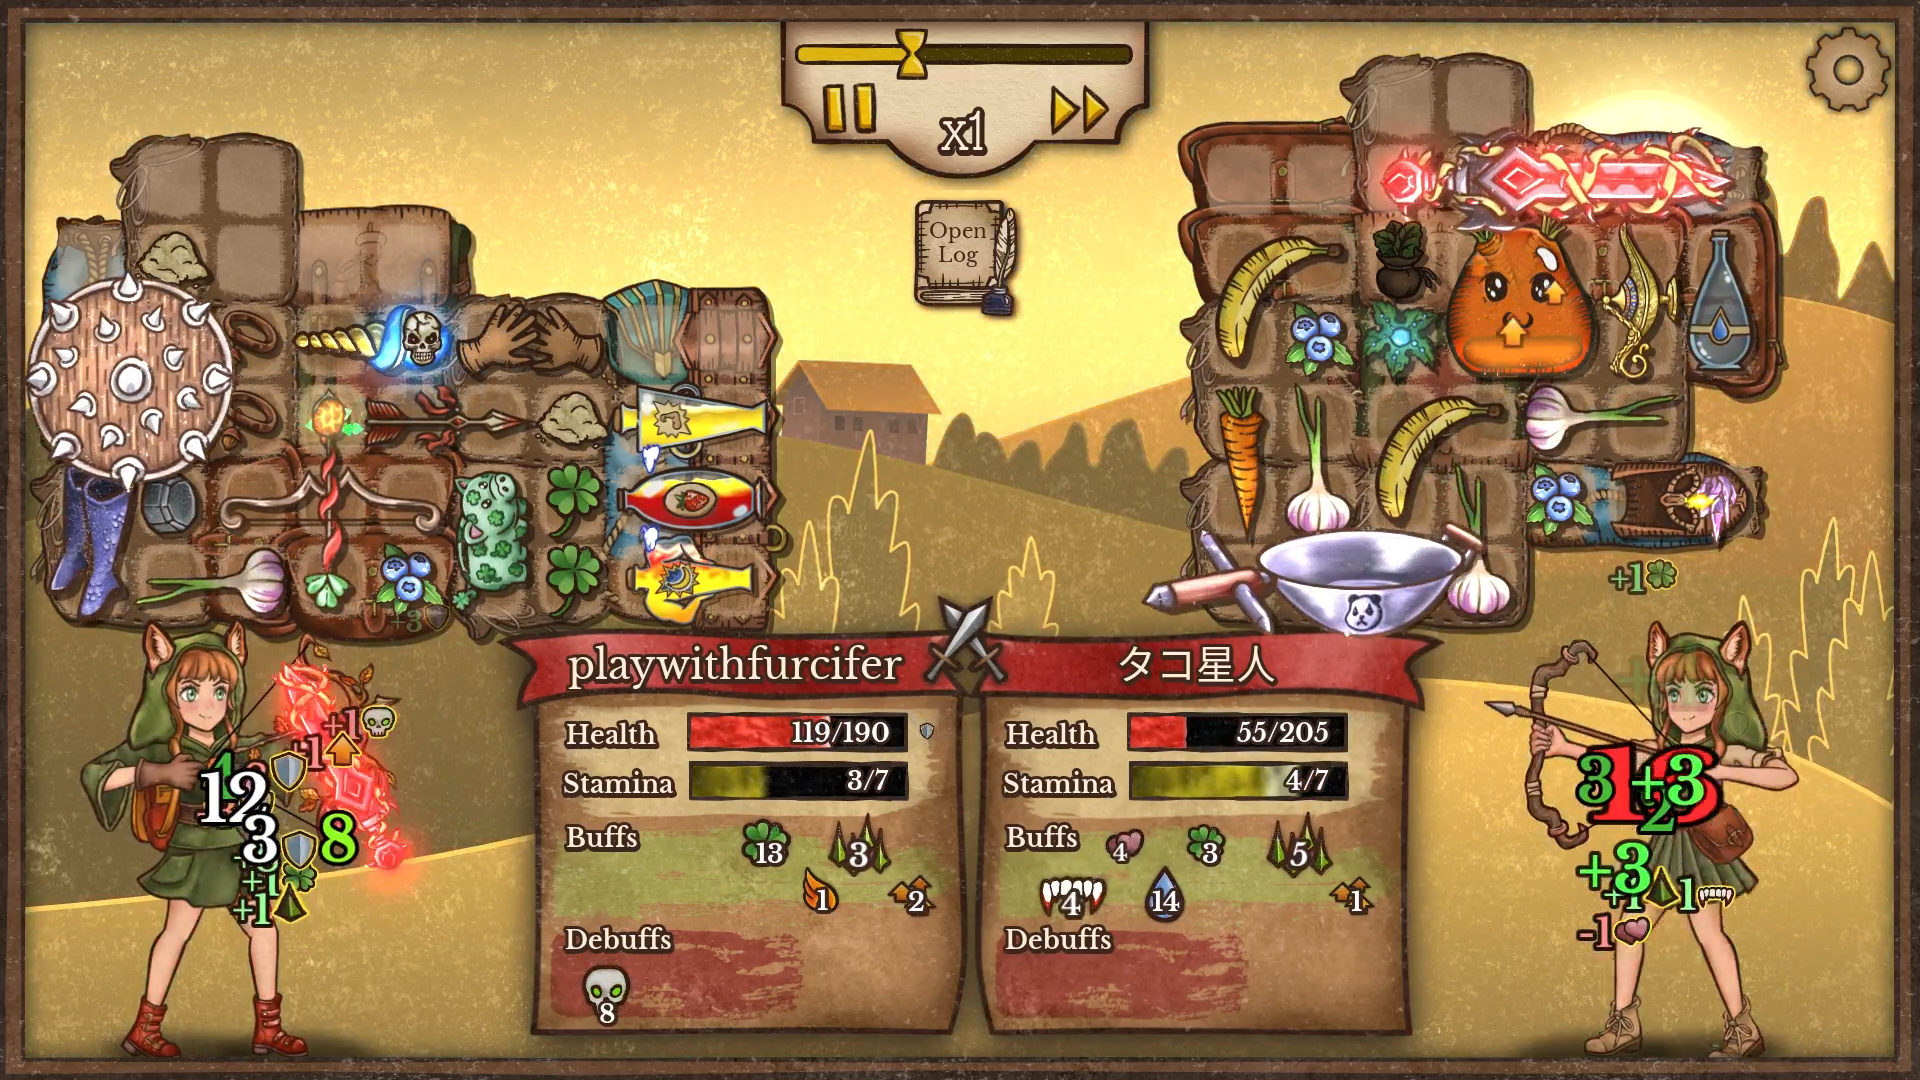
\includegraphics[width=\textwidth]{images/backpack_battle_sample.jpg}
        \caption{\textit{Backpack Battle}}
        \label{fig:backpack_battle_sample}
    \end{subfigure}
    \begin{minipage}{0.05\textwidth}
        \centering
        +
    \end{minipage}
    \begin{subfigure}{0.17\textwidth}
        \centering
        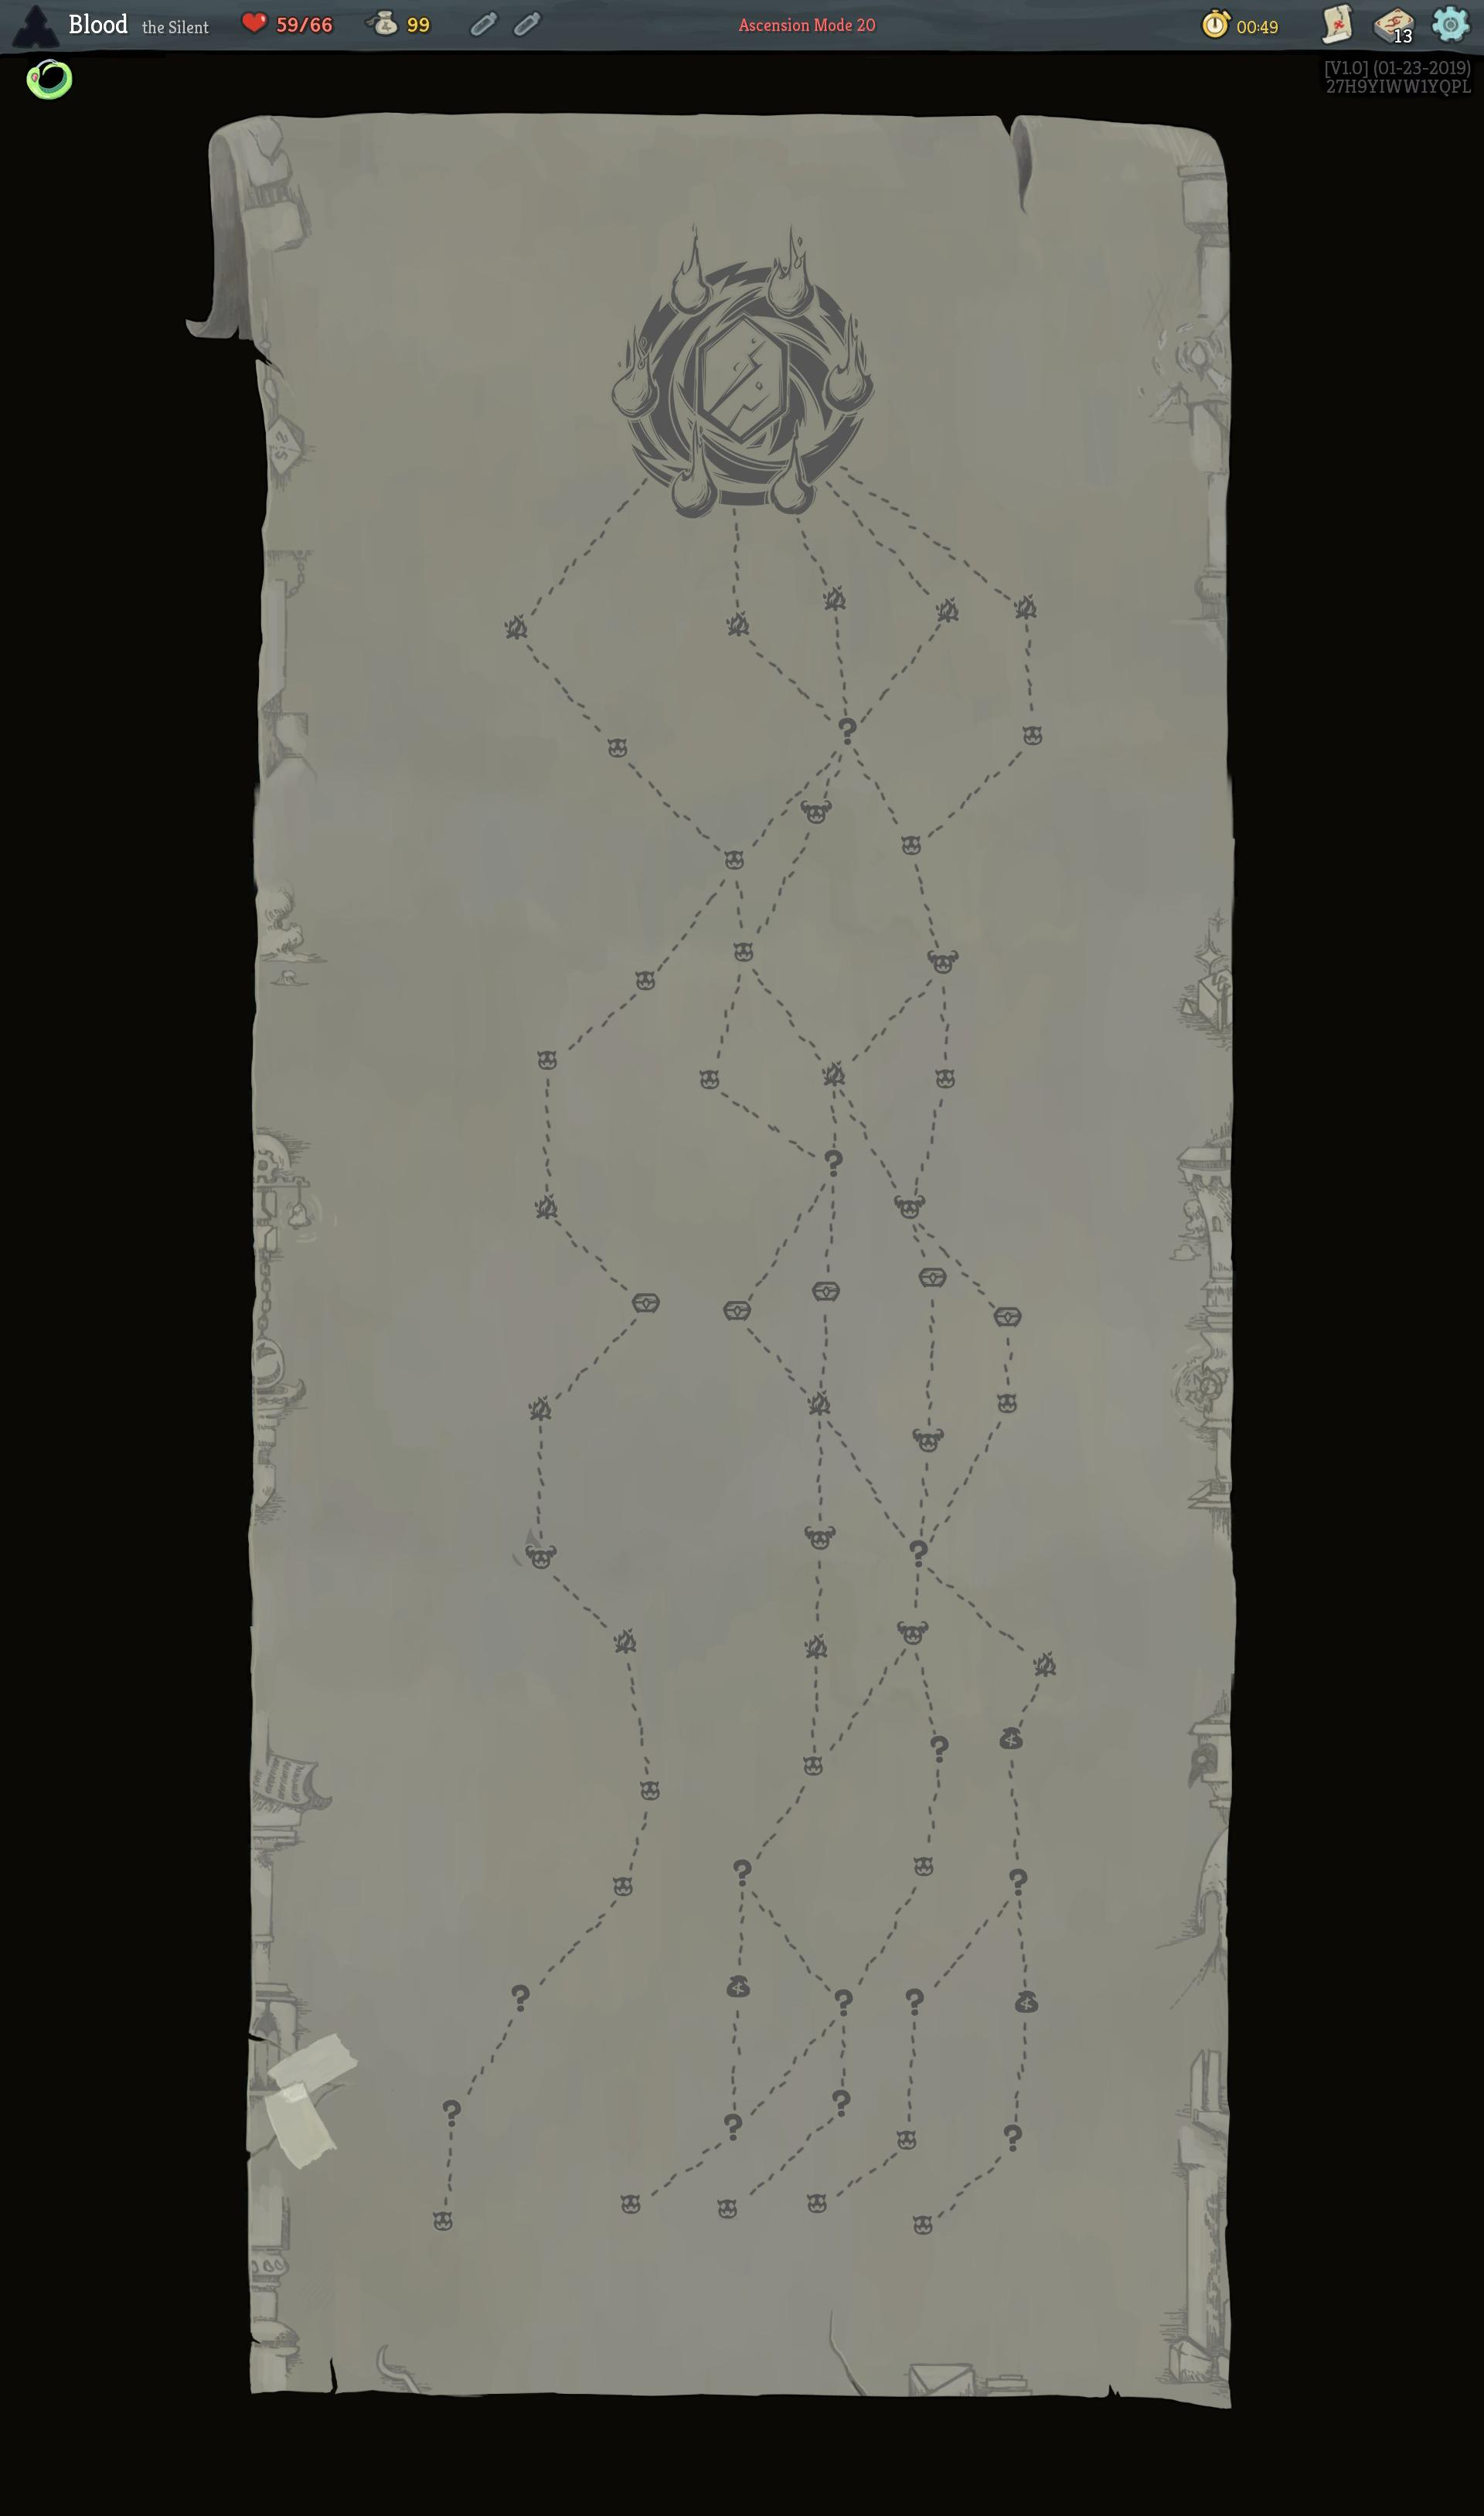
\includegraphics[width=\textwidth, height=4cm]{images/slay_the_spire_sample.jpg}
        \caption{\textit{Slay The Spire}}
        \label{fig:slay_the_spire_sample}
    \end{subfigure}
    \begin{minipage}{0.05\textwidth}
        \centering
        =
    \end{minipage}
    \begin{minipage}{0.2\textwidth}
        \centering
        \textit{SoulSwords MVP}
    \end{minipage}

    \caption{Imagens de Referência para a fase 1 (MVP)}
    \label{fig:imagens_referencia_mvp}
\end{figure}


Em uma versão futura, serão implementadas a parte 
\textit{top-down} do jogo e suas respectivas mecânicas.


\begin{figure}[!ht]
    \centering

    \begin{subfigure}{0.2\textwidth}
        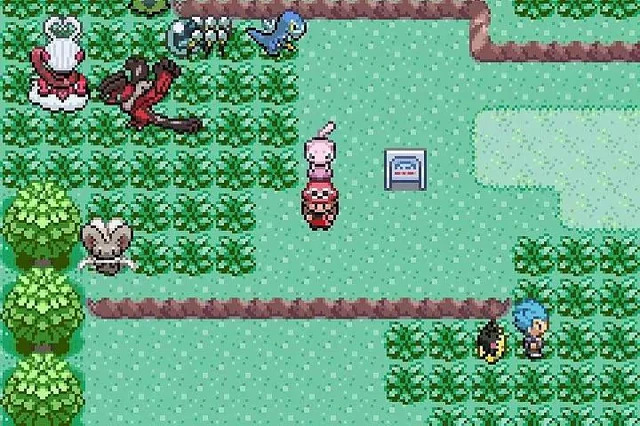
\includegraphics[width=\textwidth]{images/pokemon_sample_1.jpg}
        \caption{Pokémon}
        \label{fig:pokemon_sample}
    \end{subfigure}
    \begin{minipage}{0.1\textwidth}
        \centering
        +
    \end{minipage}
    \begin{minipage}{0.2\textwidth}
        \centering
        \textit{SoulSwords MVP}
    \end{minipage}
    \begin{minipage}{0.1\textwidth}
        \centering
        =
    \end{minipage}
    \begin{minipage}{0.16\textwidth}
        \centering
        \textit{SoulSwords}
    \end{minipage}

    \caption{Imagens de Referência para a fase 2 (Versão Final)}
    \label{fig:imagens_referencia_final}
\end{figure}